%!TEX root = uist14.tex

\section{Iteration 1: Naive IR}
Our initial research question is: {\em Can IR-based targeting reduce the selection time compared to the case where only UI list navigation is used on a head-worn device?} 

\subsection{Technique}
In our first implementation, we use IR for scanning as described in the previous section. For the refinement stage, we simply show a list of the subset of targets that have received IR signals on the Glass display. Users swipe to select from that list and tap to confirm the intended target.

A natural point of comparison is an interface that does not use any head orientation information - it always shows a complete list of all targets. We implemented a list view where users swiped forward and backward on the Glass touchpad to navigate incrementally through the list. To quantify the benefit of using IR for the scanning step, we carried out a target acquisition study which compares the {\em Naive IR selection} and {\em list selection}.  

\subsection{Method}
We deployed 10 wireless nodes in an indoor environment (Figure~\ref{fig:targeting-study-layout}). Each of them has a number as ID and a letter representing the name. We recruited 14 participants from our institution for this study. 13 had never used Google Glass before, so we offered a tutorial before the experiment in order to introduce the device. Four participants wore prescription glasses, which makes Glass more cumbersome to use and adjust, and may have affected their task performance. In this study, the IR LED was fixed and not repositionable as shown in Figure~\ref{fig:glass}.

\begin{figure}[t]
\centering
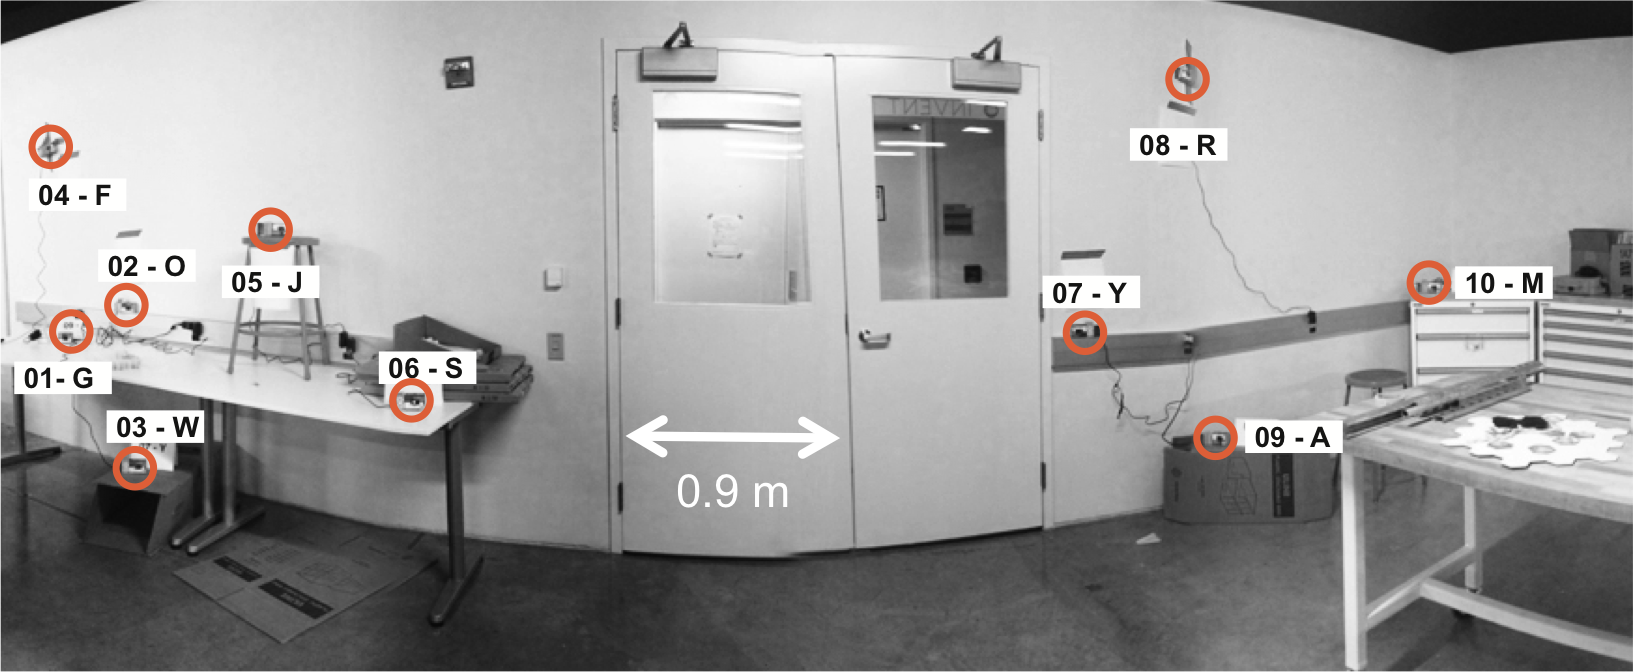
\includegraphics[width=1.0\columnwidth]{figures/study-layout1.png}
\caption{In the targeting study, participants were asked to find and select one of 10 targets in the lab environment.}
\label{fig:targeting-study-layout}
\end{figure}

In the within-subject study, half of the participants performed {\em IR selection} first and the other half used {\em list selection} first. For each selection condition, we conducted 15 target selections by randomly choosing from all the targets. During the study, we measured the {\bf target acquisition time} for each target selection. Afterward, participants were asked to complete a survey of primarily open-ended answers about their experience.

%% remove this for now
%% Our measurements suggest that IR communication can be targeted to an area about 60-120cm in diameter, up to 5m in front of the user. These values are a reasonable match for selecting targets in a room-size environment. A wider beam would lead to an increased chance of multiple appliances receiving IR signals simultaneously. A narrower beam will make targeting more challenging, given the precision constraints of human head movement.


\subsection{Results}


Our results indicate that {\em IR selection} outperforms {\em list selection}.  The average target acquisition time for {\em IR selection} is 6.67 seconds 
while {\em list selection} took 8.86 {\em list} seconds (see Figure~\ref{fig:ir_vs_list}). A t-test shows a significant difference ($t(279)=-3.81, p=0.00017$).


\begin{figure}[t]
\centering
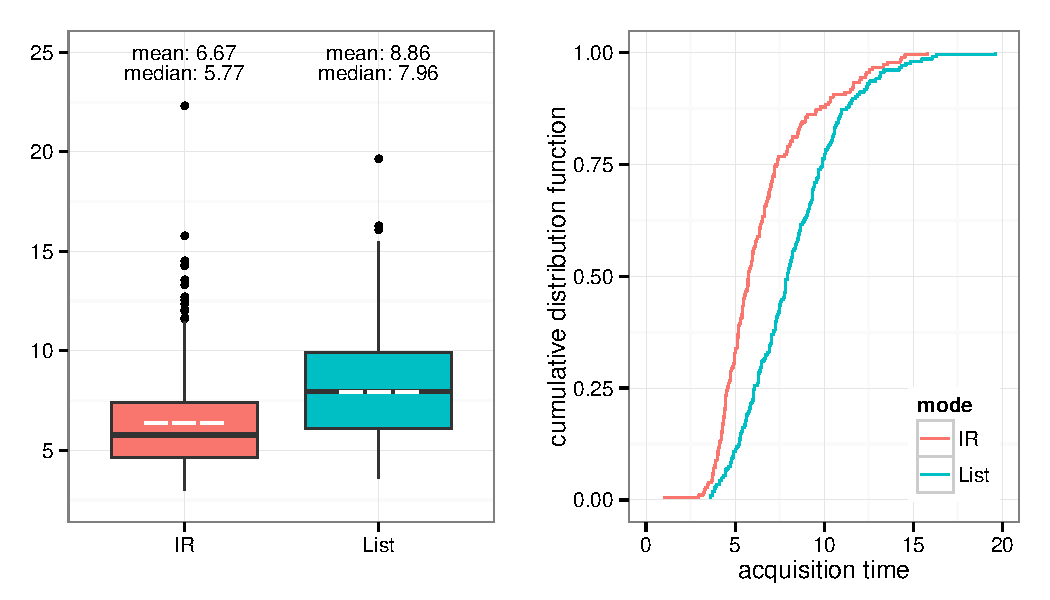
\includegraphics[width=1.0\columnwidth]{figures/result_study1a.pdf}
\caption{Boxplot of target acquisition time for {\em IR selection} and {\em list selection} is shown on the left. The center is the median value, and the mean value is shown using white dashed lines. The cumulative distributions are on the right.}
\label{fig:ir_vs_list}
\end{figure}

\begin{figure}[t]
\centering
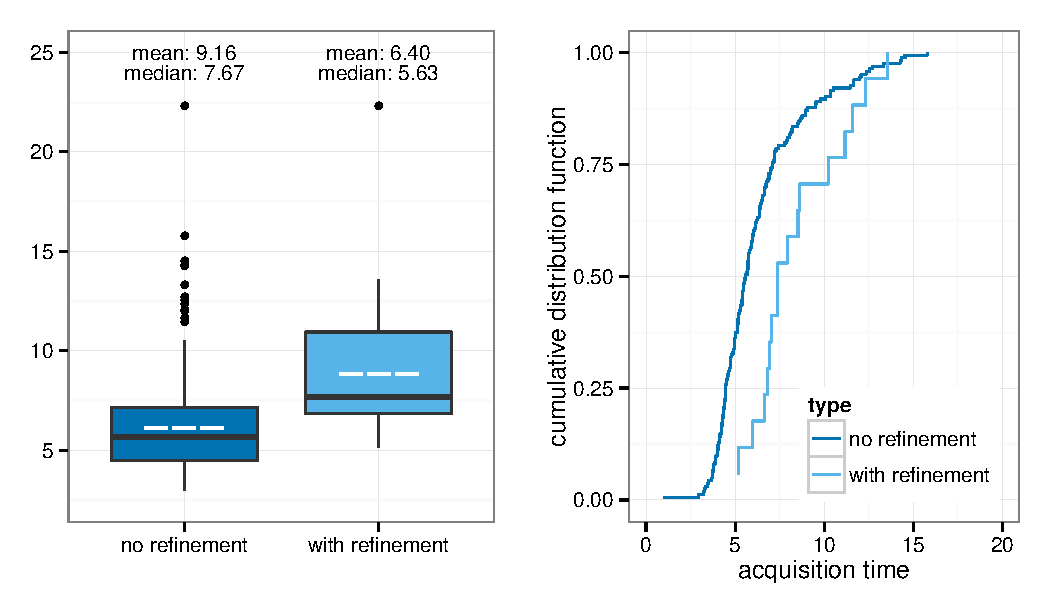
\includegraphics[width=1.0\columnwidth]{figures/result_study1b.pdf}
\caption{Boxplot and CDF of target acquisition time when refinement is needed or not in {\em IR selection}}.
\label{fig:with_without_refinement}
\end{figure}

\begin{figure}[t]
\centering
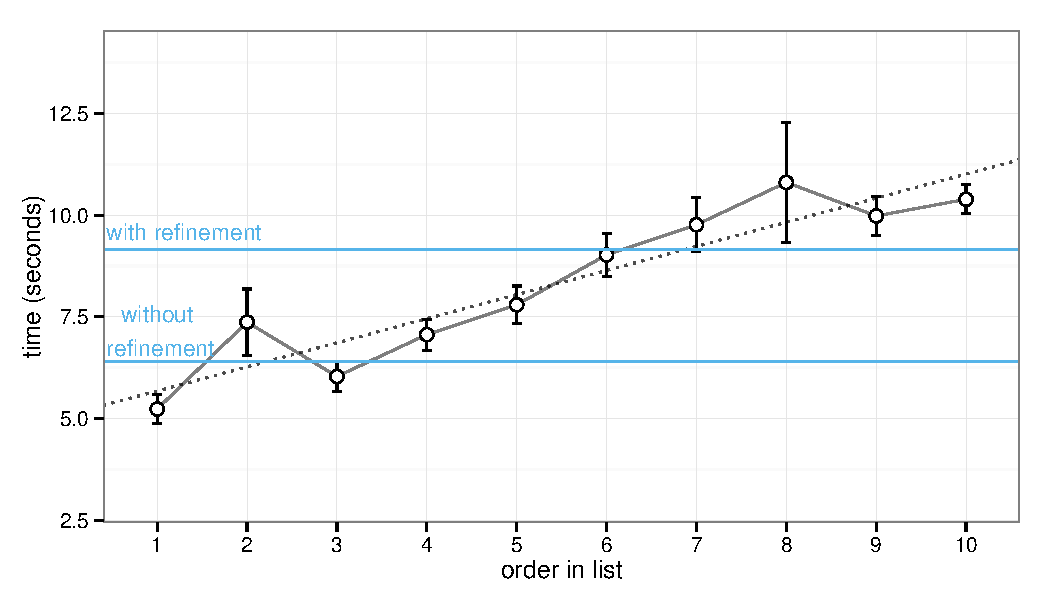
\includegraphics[width=1.0\columnwidth]{figures/result_study1c.pdf}
\caption{Times taken to select a device vs.~its order in the {\em list selection}. The dotted line is a linear fit between the average time and target orders in the list. Two horizontal solid lines are the average target acquisition times in {\em Naive IR} when refinement is needed or not.}
\label{fig:time-vs-list-order}
\end{figure}

To understand how scanning and refinement contribute to total selection time, we split the data from {\em IR selection} into two parts -- trials that required refinement and ones that did not. It takes 6.40 seconds (on average) to complete  a selection without any refinement, but 9.16 seconds with refinement, indicating that an additional 2.76 seconds are needed for disambiguation (see Figure~\ref{fig:with_without_refinement}). This difference is significant $(t(19)=-2.7827, p=0.012)$ using t-test.
%  \bjoern{I don't understand why we have 279 DF in the previous test but only 19 here??}). 
%% \ben{Because the times when refinement is needed is only 18 times, so the DF is bounded by the samples.}
Because many targets were spaced far apart, refinements were only necessary in 10\% of total {\em IR selection} trials in this study.

To further generalize the results, in Figure~\ref{fig:time-vs-list-order}, we show the acquisition time for each individual target in {\em list selection} condition, ordered by their relative position in the list. Since with IR technique, the acquisition time is invariant from each target's order, we use solid lines to represent the average performance of {\em IR selection}. From this figure, we can see that once there are more than 6 targets, the average acquisition time will be larger than IR selection, even if disambiguation is needed. %Therefore, we argue that once there are more targets in the physical space, the {\em list selection} method is not scalable. Further more, in real-life scenarios, targets would have longer names than an alphabet letter. This would increase the searching and text comparison time and also reduce the number of targets being shown in the UI screen.

As for the qualitative feedback, 11 out of 14 participants preferred IR selection over list mode (two preferred list, one was undecided). While both interfaces were judged similarly on overall ease of connecting, list selection was perceived to be cumbersome. One user noted benefit of {\em IR selection} being \studyquote{more direct [than list mode]}, allowing users to focus on the targeted objects instead of the screen. \achal{This seems rather weak... Don't really need all the quotes.} One subject called it \studyquote{natural to interact with things just by looking at them}. Another mentioned that \studyquote{it's really convenient that what I'm looking at is what I'm targeting}, and many participants compared the overall time of target acquisition. One subject pointed out that \studyquote{{\em IR selection} doesn't requires you to swipe a lot of times like list mode}.

In summary, {\em Naive IR} can outperform linear list selection, and most users prefer this head-orientation based targeting. From our quantitative result, however, we found that the refinement step detracts significantly from the efficiency of the technique.


% learned that with IR, we can have effectively reduced the overall target acquisition time. And the major gain comes from the fact that {\em coarse selection} helps reduce the chances of entering {\em fine selection} stage.

%\subsubsection{Preference}

%Eleven of 14 users preferred infrared mode over list mode (three preferred list, one was undecided). While both interfaces were judged similarly on overall ease of connecting, list navigation was also perceived to be cumbersome. As self-report data can easily skew positive as participants try to please experimenters, we also asked participants to elucidate why they preferred one interface over the other.

%List mode had certain advantages: It was judged to be more accurate and predictable as there was always exactly one device selected in the list (\studyquote{With the list you never have to worry about accidentally picking up two targets}). Also, it did not require a clear line of sight to the target device so participants did not have to move from their starting position (\studyquote{The shortcoming of the IR mode was that you had to be a certain distance away in order for it to detect the appliance}). 

%On the other hand, list mode was judged to be more \studyquote{annoying} and tedious. The temple-based touchpad for selection was difficult to use for a participant with long hair: \studyquote{List mode was physically difficult for me to navigate, since my long hair wasn't tied back and it kept interfering with my swiping.} Another participant also commented on the ergonomic challenge of touchpad use on Glass: \studyquote{The strength of the IR mode was that I didn't have to use my fingers as much to control. If the items were spaced relatively far apart, it was easy to select a specific appliance.}

%One noted benefit of infrared mode was a feeling that it was \studyquote{more direct [than list mode]}, allowing users to focus on the targeted objects instead of the screen. One subject called it \studyquote{natural to interact with things just by looking at them}. Another mentioned that \studyquote{it's really convenient that what I'm looking at is what I'm targeting}. 

%A few perceived weaknesses of infrared mode were the necessity to move the head in order to control a device and the imperfect mapping of gaze to target. One participant said that it was \studyquote{awkward to be aiming your head at things, tweaking back and forth to get it right}. Another noted that observing the head movement didn't capture the site of her attention, because \studyquote {eye movement is an important part of how people look around}. Users had to learn the usable angle of the IR emitter before they became successful at controlling the devices: \studyquote{I had to compensate by tilting my head up a little bit.}

%%% Local Variables: 
%%% mode: latex
%%% TeX-master: "uist14"
%%% End: 
